%% LaTeX2e class for student theses
%% sections/content.tex
%% 
%% Karlsruhe Institute of Technology
%% Institute for Program Structures and Data Organization
%% Chair for Software Design and Quality (SDQ)
%%
%% Dr.-Ing. Erik Burger
%% burger@kit.edu
%%
%% Version 1.3.5, 2020-06-26

\chapter{Introduction}
\label{ch:Introduction}

%% -------------------
%% | Example content |
%% -------------------

Metal Catalysts are crucial to a variety of applications, from water splitting to CO2 reduction.
% TODO: Elaborate
Catalyst are used in combination with chemical reactions to lower their activation energies.
Catalysts have an activation energy them self that needs to be overcome in oder to start the reaction.

The reaction barrier depends on the structure of the catalyst, and varies greatly between different catalyst molecules.
Intuitively no rule for the activation barrier can be found.
Seemingly small changes in the catalysts shape can have a large influence on the catalysts activation barrier \ref{fig:struct-diff}.
Knowing how to change catalyst molecules in order to lower their activation barrier is a difficult challenge, even to humans.
While the activation barrier can be computed, this process is highly complex and takes a lot of computing power.
This means computing the activation barrier for large dataset of catalysts is currently not feasible.

In this Bachelor's thesis, different approaches top use machine learning to compute the activation barrier of catalyst molecules are explored.
Different methods of encoding catalyst molecules into machine-understandable formats are proposed.
Using a combination of machine learning techniques, mostly artificial neural networks, the activation barrier is predicted from the catalysts shape.

After being able to predict the activation barrier with high accuracy, different techniques to explain machine learning results are used.
This allows for intuition of which parts of the catalyst molecule contribute to the prediction of the activation barrier.
This intuition may be helpful in further chemical analysis of the metal catalyst and can help to give the 
chemist an idea on how an element needs to be changed in oder to lower it's activation barrier.
\\


\begin{figure}
  \centering
  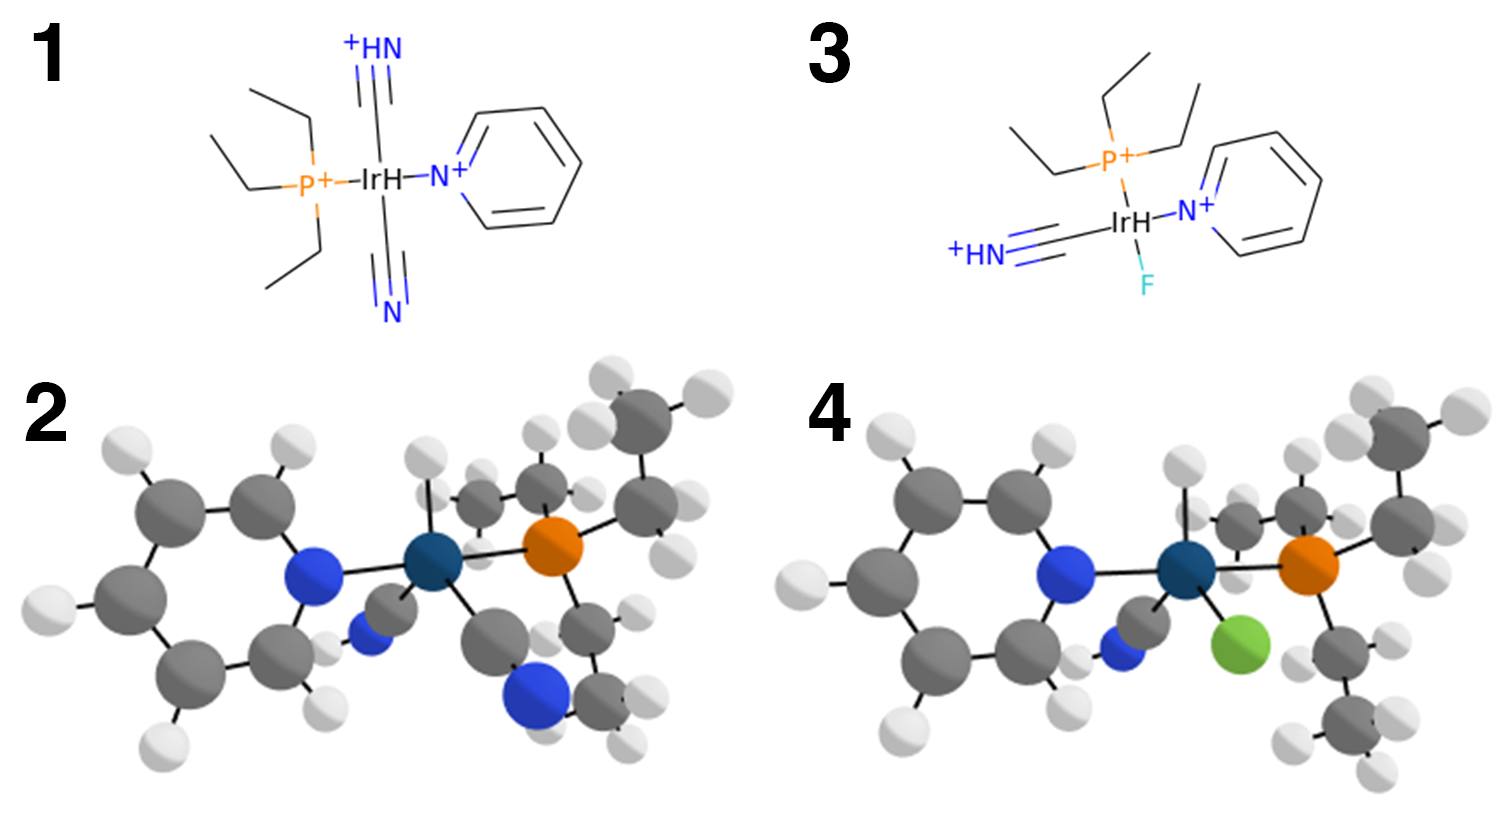
\includegraphics[width=0.8\textwidth]{figures/introduction/elems_intro.png}
  \caption{Two elements with seemingly very similar chemical structures. The chemical structure 1 and it's corresponding 3d structure 2 have an activation barrier of $3.6 kcal/mol$.
  Molecule 3 and it's corresponding 3d structure 4 have an activation barrier of $18.0 kcal/mol$.
  The only difference in the 3d structure of the 2 is the fluorine arm is being replaced by a nitrogen arm.
  The difference is significant considering the standard deviation shown in \ref{fig:barriers}.  }
  \label{fig:struct-diff}
\end{figure}


The metal catalysts used used here are constructed by combining different ligands around a central Iridium atom.
This allows for quick generation of thousands of different catalyst molecules.
By adding more ligands, the dataset can be increased in size with little effort.
For all catalysts in the dataset the activation barrier, along with other properties, is then computed.
Since calculating the activation barrier is very costly, a total of 1947 species with different structures are constructed.
\\
As with many machine learning tasks, feature selection is one of the big challenges in this project.
While there are many universal techniques to extract extract features from chemical structures, they all have their drawbacks.

In previous works, multiple different techniques are proposed to extract features from a catalyst molecule \cite{friederich_dos}.
While these techniques are based on the chemical structure of a molecule, they do not take into account its 3D spacial structure.
The feature extracting methods developed in this bachelor thesis will rely heavily on the 3D structure of molecule.
The idea being that the 3D structure plays an important role in the activation barrier, and encoding the 3D structure will enhance regression accuracy.
Additionally encoding the 3D structure will allow to learn about the space surrounding the central 
Iridium atom to understand the importance of location of the atoms in our molecule.

There currently is no widespread way to encode catalyst molecules that also allows for 
reconstruction of the 3d space and by that an intuition on how the molecule needs to be changed in order ot lower the activation barrier.
\\
The seemingly arbitrary distribution of activation barriers among catalyst molecules  was reason to use neural networks for prediction from the generated features.
Neural networks have become the go-to method for high dimensional regression and classification for their ability to adapt well to complex data.
\\
A limitation of neural networks however is their fixed-size input space.
Therefor a representation of the catalyst needs to be found that encodes our molecule into a fixed-size set of features.
These features will then be fed into our neural network for training. 
\\
3D structural encoding however comes with its own set of challenges. 
One more general being neural networks sensitivity to rotation and positioning.
Since a molecules activation barrier does not change depending on its rotation or location in space, 
information about rotation and translation should ideally not be part of the molecules features.
\\
In the case of the metal catalysts, achieving translational invariance is trivial.
Since every catalyst is constructed around exactly one metal atom, the molecule can be centered around this metal atom.

For rotational invariance the problem is more complex.
Every catalyst has a reaction pocket attached to it's cental atom.
This reaction pocket has a fixed position.
With the vector from the center of the Iridium atom to the center of the reaction pocket, two more degrees of freedom can be removed.
For the last degree of freedom, rotations around this vector, there is no natural way to get rid of it.

Here, 2 different approaches to this last degree of freedom are explored.
The first is a rotationally invariant description using fourier coefficients.

The second is using data augmentation to teach the neural network about all possible rotations.
This means the molecule is rotated along the last remaining axis of freedom, and and multiple examples of the same molecule at different rotations are used as training examples for the neural network.
This ideally allows the network to learn the molecules structure independent of it's rotation.


\section{Dataset}

The dataset contains 1947 examples of catalyst molecules.
For each atom of the molecule, the location in space is given.
For each molecule it's activation barrier is known.

\begin{figure}
  \centering
  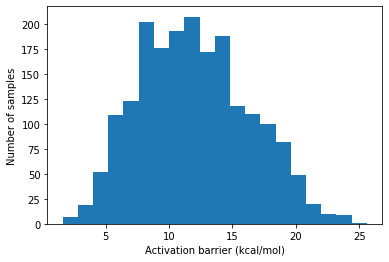
\includegraphics[width=7cm]{figures/introduction/barrier.png}
  \caption{Distribution of the elements activation barrier. The elements have a mean of $11.970 kcal/mol$ and a standart deviation of $4.33 kcal/mol$.}
  \label{fig:barriers}
\end{figure}

The molecules were generated by combining ligands around a central Iridium atom as illustrated in \autoref{fig:chemspace}.
The activation barrier was then calculated.
Due to this combinatorial approach the dataset could later be increased with relatively low effort \ref{fig:chemspace}.
Together this gives a dataset containing the structure and the associated activation barrier for 1947 Iridium catalysts.

\begin{figure}
  \centering
  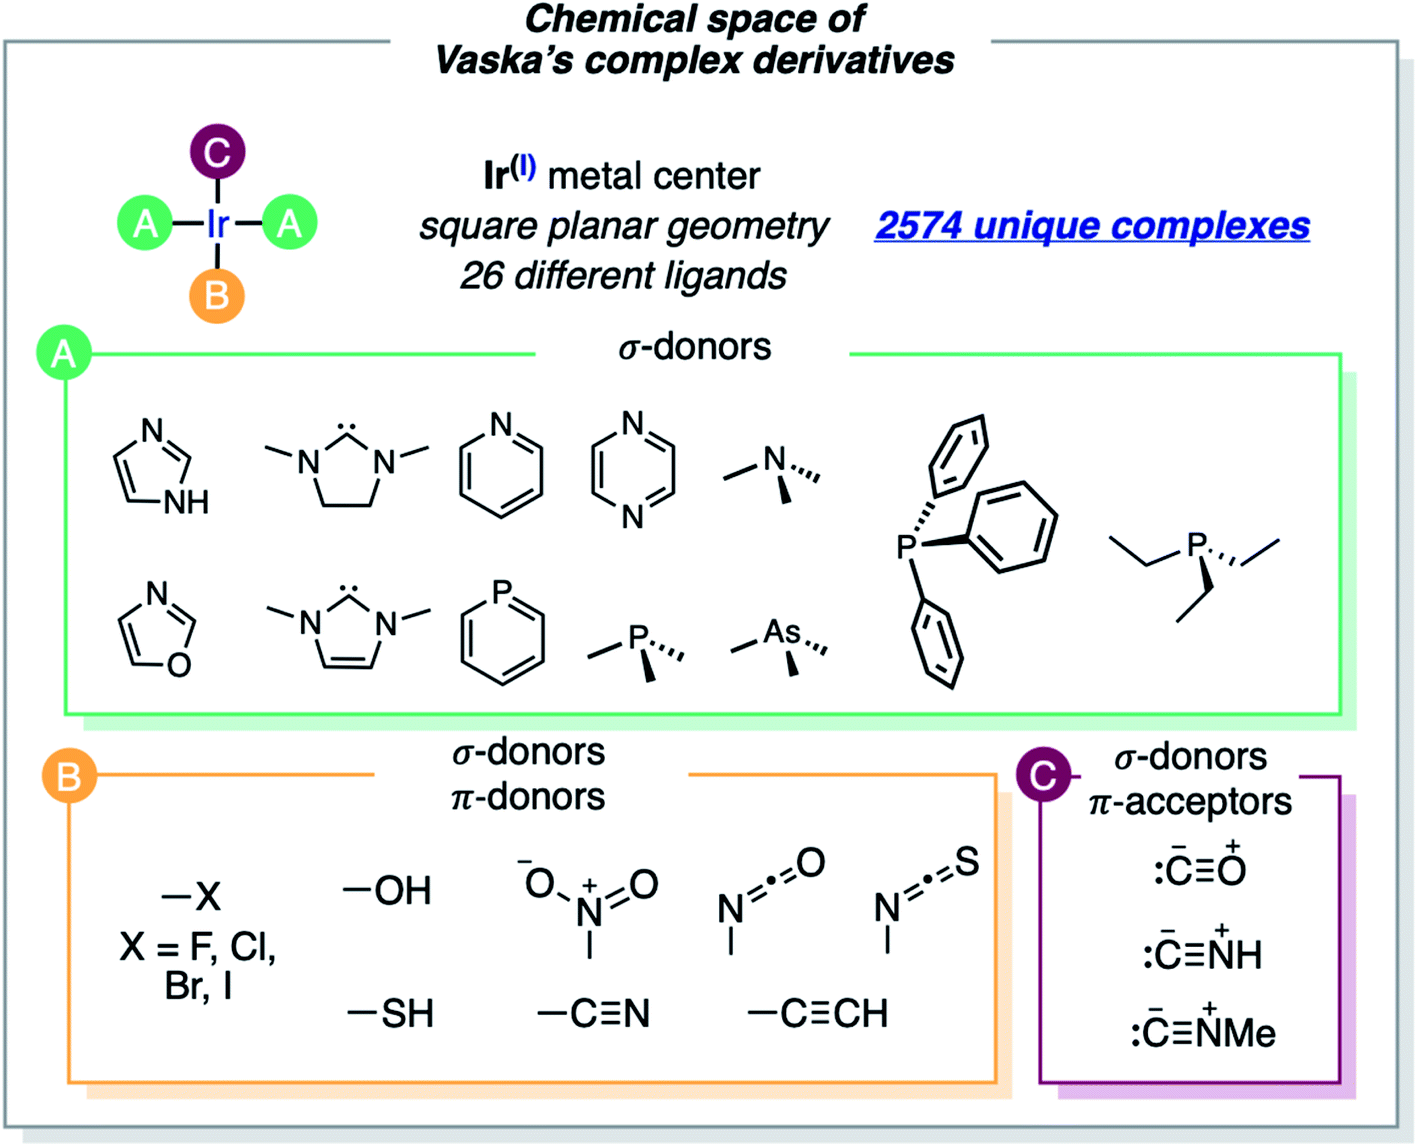
\includegraphics[width=10cm]{figures/introduction/chem-space.png}
  \caption{Ligands defining the chemical space associated with Vaska's complex. Reprinted from \cite{friederich_dos}.}
  \label{fig:chemspace}
\end{figure}

When examining the dataset by hand, the connection between a molecules structure and it's activation barrier is not obvious.
Seemingly small changes can have a big influence on it's activation barrier.

A rule to guess the activation barrier from the molecules structure can not easily be found.

Every single element in the dataset has consist of a number of atoms.
The number of atoms forming one molecule varies between elements.
Each atom has a unique position, other chemical properties can be associated with the atom, such as atmoic radius, eleoctromagnetivity and many more.
The location and rotation of the elements in the dataset is seemingly arbitrary.
Note that the global location and rotation of the molecule does not influnce it's activation barrier.
Local changes in atomic position however can have effects on the activation barrier and other properties of the molecule.
  

\section{Previous research}

In previous approaches different machine learning methods were used to predict the activation barrier of elements.
However, the features extracted from the molecule did not take into account the spacial structure of the element.
The elements were instead encoded by creating a graph from the chemical structure.
The elements are then grouped by their distance from the metal center.
For each group of elements, different features are computed as sum of pairwise products/differences of their atomic properties(such as electronegativity, atomic number, identity, topology and size) \cite{friederich_dos}.
Note that these features do not contain any information about the 3D location of the atoms.

Using these autocorrelation features, a neural network and gaussian processes and other forms of regression were used to predict the activation barrier.
Neural networks and gaussian processes both were able to predict the activation barrier within an error of $<1 kcal/mol$ for a test split of $10\%$

Other than the obvious disadvantage of not encoding location information, another disadvantage is the lack of interpretability of results.
While these features succeed at predicting reaction barriers, information what part of the molecule is contributing to the prediction is limited.

The feature extractors introduced in this thesis aim to solve this problem by extracting features that allow for a
partly reconstruction of the chemical space and thus knowing which region of the molecule contributes to a prediction.

Feature extraction is a common problem for machine learning methods in chemical spaces.
Multiple approaches have been proposed for general molecule encoding, 
ranging from encoding properties of molecules, such as the Coulomb Matrix encoder encoding electrostatic interaction of atoms \cite{PhysRevLett.108.058301}
to encoding 3D structures of atomic environments \cite{Bart_k_2013}.

3d structural encoders usually create a fully invariant features description.
In the case of SOAP proposed by \citeauthor{Bart_k_2013}, this is achieved by encoding information about the interaction of 
different species rather than encoding the 3d space itself.
Fully invariant 3d descriptors have the advantage of being universally applicable for any kind of molecule, since they have no requirements to the element being encoded.
The disadvantages are that, once the features are generated, a transformation back to 3D space is not possible.
In many applications, this is not a problem since the generated features are used only for prediction of an elements properties.
In our case, the features however should later allow us to interpret the 3D space surrounding the molecule and ideally give an idea on how the molecule can be changed to alter it's properties.

The idea of using a catalysts special structure for this task, and therefor removing some axes of freedom from the feature space, seems to be an unexplored approach.

Since the structure of the catalyst still leaves 1 degree of freedom, the prediction needs to be partly rotationally invariant.
This is a common problem for neural networks even outside of chemistry.
Generally the approaches to solving these problems can be divided into 2 different groups.

The first being feature engineering to generate features from the data that is fully invariant of rotation.
In point clouds approaches include representating the data as angles and distances rather than the points itself \cite{8886052,weiler20183d}.
Since these features do not change depending on the rotation and translation of the points, the network does no need to 
abstract away the rotational information of the data.
While this method guarantees full rotational invariance, it requires extensive feature engineering.
Some local rotations that might be helpful to the neural network can also go missing. %TODO: Remove?
The EFD feature generator proposed here implements a fully rotationally invariant description by using 
descriptor that can be normalized for rotation.

A second approach to rotational invariance is data augmentation.
In image recognition data augmentation has already become the go-to method.
Data augmentation removes the need for extensive feature engineering.
Instead, the training data is augmented along all axes of freedom.
In the case of image recognition, this means rotating, scaling, and in some cases deforming the input images.
By that, the dataset will be filled with more examples for every datapoint, and the model is will be able to learn to 
abstract away these features. %TODO: Citation needed
The SNAP feature generator proposed here produces a partially rotationally invariant output that needs to be augmented along one axis.
All the augmentation steps are then fed to the networks in order to teach the network to abstract away the different rotations of the catalyst.

\section{Objectives}

This work can be grouped into 2 main objectives. 
The first is to find a feature extractor that generates features from a catalyst molecule that ideally rotationally invariant.
The second objective is to train a neural network on these features that predicts the activation barrier.
The goal was to achieve accuracy similar or higher to what \citeauthor{friederich_dos} achieved in \cite{friederich_dos}.
In a final step, using explainers to explain the origins of the networks prediction, an intuition on how a catalyst has 
to be adapted in order to change it's activation barrier is given.

\subsection{Feature generation}

The features should allow a regressor to make predictions from the euclidean space surrounding the central Iridium atom.
Therefor features have to be of fixed length for all elements in the dataset.
Ideally the number of features is as low as possible, helping the model to identify the relevant features better.
For interpretability of the results, the features should allow for a partial or full reconstruction of the euclidean space they are encoding.
This means, given the features, it should be possible to approximate the general shape of the molecule.

The global location and rotation of the element should not influence the features or have only limited influence on the features.

Two different approaches to feature generation are prosed.
The first is a fully rotationally invariant output using a rotationally invariant contour description.
While the output of this descriptor is fully invariant, it suffers from sampling issues due to the nature of it's encoding.

The second approach to feature generation was using a combination of basis functions to fully construct a local SE(3) environment around the central atom.
Using a set of coefficients, the density space surrounding the central atom can be approximated.

\subsection{Regression}

The second step is to predict the activation barrier from these features using an artificial neural network.
The goal was to find a network able to to predict the activation barrier with accuracy similar or better to the machine learning methods proposed by \citeauthor{friederich_dos}.
The networks proposed here achieve higher accuracy's than all the best regression methods proposed in \cite{friederich_dos}.

Especially the regression methods performed on SNAP features achieve accuracies significantly higher than regression methods on graph convolutions.

\subsection{Explaining the feature space}
Since the features should be able to allow a inversion back to the 3D space, it's possible to approximate which areas in 3D space are responsible for the prediction.
Using neural networks explainers, in  a last step the regions in 3d space that influence the regression will be analyzed.
This gives an idea on how different atoms in the dataset influence the prediction.
Looking at the gradient of the input with respect to the activation barrier, an intuition on how the catalyst molecule needs to be 
adapted in order to decrease the activation barrier can be given.
